\chapter{Learning问题}

在Evaluation问题中,我们在已知模型$\lambda$的情况下,基于前向算法或者后向算法
可以得出观测序列的联合概率分布$P(O|\lambda)$。而Learning问题就是在已知观测数据
的情况下求参数$\lambda$。

\begin{equation}
    \lambda_{MLE}=\arg \max\limits_{\lambda}P(O|\lambda)
\end{equation}

\section{Learning}

我们需要计算的目标是
\begin{equation}
    \lambda_{MLE}=\arg\max_{\lambda}P(O|\lambda)
\end{equation}

联合概率分布表示为
\begin{equation}
    P(O|\lambda)=\sum_{I_1}\cdot\sum_{I_2}\cdot\cdots\cdot \sum_{I_T}\pi_{i_1}\prod_{t=2}^{T}a_{i_t-1,i_t}\prod_{t=2}^{T}b_{i_t}(O_t)
\end{equation}

直接计算非常困难,因此考虑使用\textsl{EM算法}。即
\begin{equation}
    \theta^{(t+1)}=\arg\max_{\theta} \int_{z}log P(X,Z|\theta)\cdot P(Z|X,\theta^{(t)})dz
\end{equation}

这里$X$替换为观测表量$O$,$Z$替换为隐变量$I$,$\theta$替换参数$\lambda$,并且注意到情况是离散的,所以

\begin{equation}
    Q(\lambda,\lambda^{(t)}) = \sum_{I} log P(O,I|\lambda)\cdot P(I|O,\lambda)
\end{equation}

\begin{equation}
    \lambda^{(t+1)}=\arg\max_{\lambda} Q(\lambda,\lambda^{(t)})
\end{equation}

\textsl{EM算法}就是最大化$Q$函数。代入联合分布概率$P(O,I|\lambda)$有
\begin{equation}
    Q(\lambda,\lambda^{(t)}) = \sum_{I} \left[\left(log \pi_{i_1}+\sum_{t=2}^{T}log\ a_{i_{t-1},i_t}+\sum_{t=2}^{T}log\ b_{i_t}(O_t)\right)\cdot P(O,I|\lambda^{(t)})\right]
\end{equation}

\section{Baum-Welch Algorithm}

得到了$Q$函数,learning问题的下一步就是极大化这个$Q$函数,求模型的参数$\lambda=(\pi,\mathcal{A},\mathcal{B})$。$Q$函数稍微做一下变化
\begin{equation}
    Q(\lambda,\lambda^{(t)}) = (\sum_{I} \left[log \pi_{i_1}\right]+\sum_{I} \left[\sum_{t=2}^{T}log\ a_{i_{t-1},i_t}\right]+\sum_{I} \left[\sum_{t=2}^{T}log\ b_{i_t}(O_t)\right])\cdot P(O,I|\lambda^{(t)})
\end{equation}

可以发现$\lambda$的三个参量$\pi,\mathcal{A},\mathcal{B}$分别都是独立的,我们可以分开求解。以$\pi^{(t+1)}$为例
\begin{equation}
    \pi^{(t+1)}=\arg\max \sum_{I} \left[log \pi_{i_1}\cdot P(O,I|\lambda^{(t)})\right]
\end{equation}

下面来计算这个式子

\begin{equation}
    \begin{aligned}
        \pi^{(t+1)}&=\arg\max \sum_{i_1}\cdots \sum_{i_T} log\ \pi_{i_1}\cdot P(O,i_1,\cdots,i_T|\lambda^{(t)})\\
    \end{aligned}
\end{equation}

联合概率分布的求和可以得到边缘概率,所以

\begin{equation}
    \begin{aligned}
        \pi^{(t+1)}&=\arg\max \sum_{i_1} log\ \pi_{i_1}\cdot P(O,i_1=q_i|\lambda^{(t)})\\
    \end{aligned}
\end{equation}

同时还有约束条件
\begin{equation}
    \sum_{i=1}^{N}\pi_i=1
\end{equation}

那么自然根据拉格朗日乘子法,构造损失函数
\begin{equation}
    \mathcal{L}(\pi,\eta)=\sum_{i_1} log\ \pi_{i_1}\cdot P(O,i_1=q_i|\lambda^{(t)})+\eta\left(\sum_{i=1}^{N}\pi_i-1\right)
\end{equation}

求解该拉格朗日函数的极值可以得出
\begin{equation}
    \pi^{(t+1)}_i=\frac{P(O,i_1=q_i|\lambda^{(t)})}{P(O|\lambda^{(t)})}
\end{equation}

这样我们就能推出$\pi^{(t+1)}=(\pi^{(t+1)}_1,\cdots,\pi^{(t+1)}_N)$,对于$\mathcal{A}^{(t+1)}$和$\mathcal{B}^{(t+1)}$也是同样的过程,因此不在赘述。

\begin{figure}[H]
    \centering
    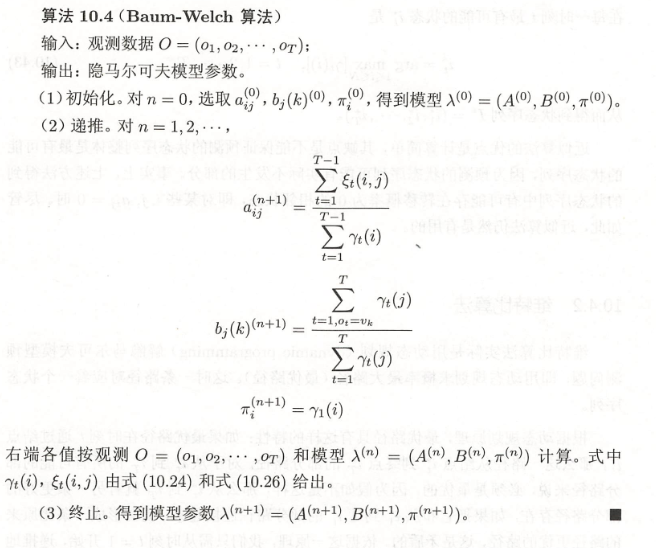
\includegraphics[scale=0.7]{figures/Baum-Welch算法.png}
\end{figure}